% Foliensatz: "AFu-Kurs nach DJ4UF" von DK0TU, Amateurfunkgruppe der TU Berlin
% Lizenz: CC BY-NC-SA 3.0 de (http://creativecommons.org/licenses/by-nc-sa/3.0/de/)
% Autoren: Martin Deutschmann
% Korrekturen: Lars Weiler <dc4lw@darc.de>, Sebastian Lange <dl7bst@dk0tu.de>

\documentclass[aspectratio=169]{beamer}

\usepackage[ngerman]{babel} % deutsche Worttrennung etc.
\usepackage[utf8]{inputenc} % UTF8 Text

\usepackage[super, comma, numbers, square, sort]{natbib}

\usepackage{hyperref}       % Hyperref Package für bessere Referenzen (todo)
\hypersetup{
	colorlinks=false,       %   false: boxed links; true: colored links
    %linkcolor=white,       %   color of internal links (change box color with linkbordercolor)
    citecolor=red,          %   color of links to bibliography
    filecolor=white,        %   color of file links
    urlcolor=blue           %   color of external links
}

\usepackage{multirow}
\usepackage{wasysym}  % Math Symbols like \permil
%\usepackage{colortbl}
%\usepackage{subscript}
%\usepackage{caption}
%\usepackage{setspace}
%\usepackage{xcolor}        % benutze CodeListe

% Footnote
%\usepackage{hanging}
%
%\setbeamertemplate{footnote}{%
%  \hangpara{2em}{1}%
%  \makebox[2em][l]{\insertfootnotemark}\footnotesize\insertfootnotetext\par%
%}


%\usepackage{pgf}
%\usepackage{tikz}
%\usetikzlibrary{arrows,automata}
%\usetikzlibrary{positioning}
%
%\tikzset{
%    state/.style={
%           rectangle,
%           rounded corners,
%           draw=black, very thick,
%           minimum height=2em,
%           minimum width=2pt,
%           inner sep=2pt,
%           text centered,
%           },
%}

%\usepackage{listings}
%\lstset{basicstyle=\small, numberstyle=\tiny, extendedchars=true, numbers=left, numbersep=5pt}
%\lstset{showtabs=false, showspaces=false, showstringspaces=false}
%%\lstset{backgroundcolor=\color{white!75!lightgray}, , frame=single}
%%\lstset{backgroundcolor=\color{white}}
%%\lstset{backgroundcolor=none}
%\lstset{keywordstyle=\color{blue!50!gray},  identifierstyle=\color{black}}
%\lstset{commentstyle=\color{green!50!gray}, stringstyle=\color{red!50!gray}}
%\lstset{language=C, fontadjust=true, tabsize=2, breaklines=true}
%\lstset{backgroundcolor=\color{white!75!lightgray}, caption=\lstname, frame=single}
%\lstset{emphstyle=\color{black}\fbox}
%
%% Keine "Listing:"-Caption
%\captionsetup{labelformat=empty,labelsep=none}
%
%% für mathematische Umgebungen
%\usepackage{amsmath,amsfonts,amssymb}
%
%\lstdefinestyle{Bash}{
%language=Bash,
%frame=single,
%rulecolor=\color{black},
%backgroundcolor=\color{gray!50},
%keywordstyle=\color{black},
%identifierstyle=,
%commentstyle=\color{black},
%stringstyle=\color{magenta!65!white},
%showstringspaces=false,
%basicstyle=\footnotesize\ttfamily\color{black},
%numbers=none,
%breaklines=true,
%captionpos=b
%}

%\usepackage{listings}
%
%\lstdefinestyle{basic}{
%    captionpos=t,%
%    basicstyle=\footnotesize\ttfamily,%
%    numberstyle=\tiny,%
%    numbers=left,%
%    stepnumber=1,%
%    frame=single,%
%    showspaces=false,%
%    showstringspaces=false,%
%    showtabs=false,%
%    %
%    keywordstyle=\color{blue},%
%    identifierstyle=,%
%    commentstyle=\color{gray},%
%    stringstyle=\color{magenta}%
%}



% fließende Boxen haben keinen Abstand
%\fboxsep0mm

% inkludiere Creative Commons Helper
%%%%%%%%%%%%%%%%%%%%%%%%%%%%%%%%%%%%%%%%%%%%%%%%%%%%%%%%%%%%%%%%
%% ccBeamer 0.1, 2007-07-02                                   %%
%% Written by Sebastian Pipping <webmaster@hartwork.org>      %%
%% ---------------------------------------------------------- %%
%% Licensed under Creative Commons Attribution-ShareAlike 3.0 %%
%% http://creativecommons.org/licenses/by-sa/3.0/             %%
%%%%%%%%%%%%%%%%%%%%%%%%%%%%%%%%%%%%%%%%%%%%%%%%%%%%%%%%%%%%%%%%


%% Images
\newcommand{\CcImageBy}[1]{%
	
\includegraphics[scale=#1]{texdata/creative_commons/cc_by_30.pdf}%
}
\newcommand{\CcImageCc}[1]{%
	
\includegraphics[scale=#1]{texdata/creative_commons/cc_cc_30.pdf}%
}
\newcommand{\CcImageDevNations}[1]{%
	
\includegraphics[scale=#1]{texdata/creative_commons/cc_dev_nations_30.pdf}%
}
\newcommand{\CcImageNc}[1]{%
	
\includegraphics[scale=#1]{texdata/creative_commons/cc_nc_30.pdf}%
}
\newcommand{\CcImageNd}[1]{%
	
\includegraphics[scale=#1]{texdata/creative_commons/cc_nd_30.pdf}%
}
\newcommand{\CcImagePd}[1]{%
	
\includegraphics[scale=#1]{texdata/creative_commons/cc_pd_30.pdf}%
}
\newcommand{\CcImageSa}[1]{%
	
\includegraphics[scale=#1]{texdata/creative_commons/cc_sa_30.pdf}%
}
\newcommand{\CcImageSampling}[1]{%
	
\includegraphics[scale=#1]{texdata/creative_commons/cc_sampling_30.pdf}%
}
\newcommand{\CcImageSamplingPlus}[1]{%
	
\includegraphics[scale=#1]{texdata/creative_commons/cc_sampling_plus_30.pdf}%
}


%% Groups
\newcommand{\CcGroupBy}[2]{% zoom, gap
	\CcImageCc{#1}\hspace*{#2}\CcImageBy{#1}%
}
\newcommand{\CcGroupByNc}[2]{% zoom, gap
	\CcImageCc{#1}\hspace*{#2}\CcImageBy{#1}\hspace*{#2}\CcImageNc{#1}%
}
\newcommand{\CcGroupByNcNd}[2]{% zoom, gap
	\CcImageCc{#1}\hspace*{#2}\CcImageBy{#1}\hspace*{#2}\CcImageNc{#1}\hspace*{#2}\CcImageNd{#1}%
}
\newcommand{\CcGroupByNcSa}[2]{% zoom, gap
	\CcImageCc{#1}\hspace*{#2}\CcImageBy{#1}\hspace*{#2}\CcImageNc{#1}\hspace*{#2}\CcImageSa{#1}%
}
\newcommand{\CcGroupByNd}[2]{% zoom, gap
	\CcImageCc{#1}\hspace*{#2}\CcImageBy{#1}\hspace*{#2}\CcImageNd{#1}%
}
\newcommand{\CcGroupBySa}[2]{% zoom, gap
	\CcImageCc{#1}\hspace*{#2}\CcImageBy{#1}\hspace*{#2}\CcImageSa{#1}%
}
\newcommand{\CcGroupDevNations}[2]{% zoom, gap
	\CcImageCc{#1}\hspace*{#2}\CcImageDevNations{#1}%
}
\newcommand{\CcGroupNcSampling}[2]{% zoom, gap
	\CcImageCc{#1}\hspace*{#2}\CcImageNc{#1}\hspace*{#2}\CcImageSampling{#1}%
}
\newcommand{\CcGroupPd}[1]{% zoom
	\CcImagePd{#1}%
}
\newcommand{\CcGroupSampling}[1]{% zoom
	\CcImageSampling{#1}%
}
\newcommand{\CcGroupSamplingPlus}[1]{% zoom
	\CcImageSamplingPlus{#1}%
}


%% Text
\newcommand{\CcLongnameBy}{Attribution}
\newcommand{\CcLongnameByNc}{Attribution-NonCommercial}
\newcommand{\CcLongnameByNcNd}{Attribution-NoDerivs}
\newcommand{\CcLongnameByNcSa}{Attribution-NonCommercial-ShareAlike}
\newcommand{\CcLongnameByNd}{Attribution-NoDerivs}
\newcommand{\CcLongnameBySa}{Attribution-ShareAlike}

\newcommand{\CcNote}[1]{% longname
	This work is licensed under the \textit{Creative Commons #1 3.0 License}.%
}


% generelles Thema auswählen
\usetheme{Goettingen} %Berlin spart ohne Sidebar allerdings angenehm Platz
% AnnArbor | Antibes | Bergen | Berkeley | Berlin | Boadilla | boxes | CambridgeUS | Copenhagen | Darmstadt | default | Dresden | Frankfurt | Goettingen | Hannover | Ilmenau | JuanLesPins | Luebeck | Madrid | Malmoe | Marburg | Montpellier | PaloAlto | Pittsburgh | Rochester | Singapore | Szeged | Warsaw

% Farben wählen
\usecolortheme{beetle}
% beaver | beetle | crane | default | dolphin | dove | fly | lily | orchid | rose | seagull | seahorse | sidebartab | structure | whale | wolverine

% Setze alle Farben auf Grau und Weiß
%\definecolor{craneorange}{RGB}{64,64,64}
%\definecolor{craneblue}{RGB}{255,255,255}

% Schriftart wählen
\usefonttheme{default}
% default | professionalfonts | serif | structurebold | structureitalicserif | structuresmallcapsserif

% Innere Themen(Kopf-, Fuß-, Sidebar usw)
%\useinnertheme{default}
\useinnertheme{circles}
% default | inmargin | rectangles | rounded | circles

% Äußere Themen (Anordnung der inneren, grenzen der Folien etc.)
\useoutertheme{infolines}
% default | infolines | miniframes | shadow | sidebar | smoothbars | smoothtree | split | tree

% Deaktiviere Navigations-Symbole ({} -> leer)
\setbeamertemplate{navigation symbols}{}
%\setbeamertemplate{navigation symbols}{\large \ifnum \insertframenumber <10 0\fi\insertframenumber/\inserttotalframenumber\vspace*{0.2ex}}

% Zeige ein Hintergrundbild
\setbeamertemplate{background canvas}{
        \hspace*{-2.0cm}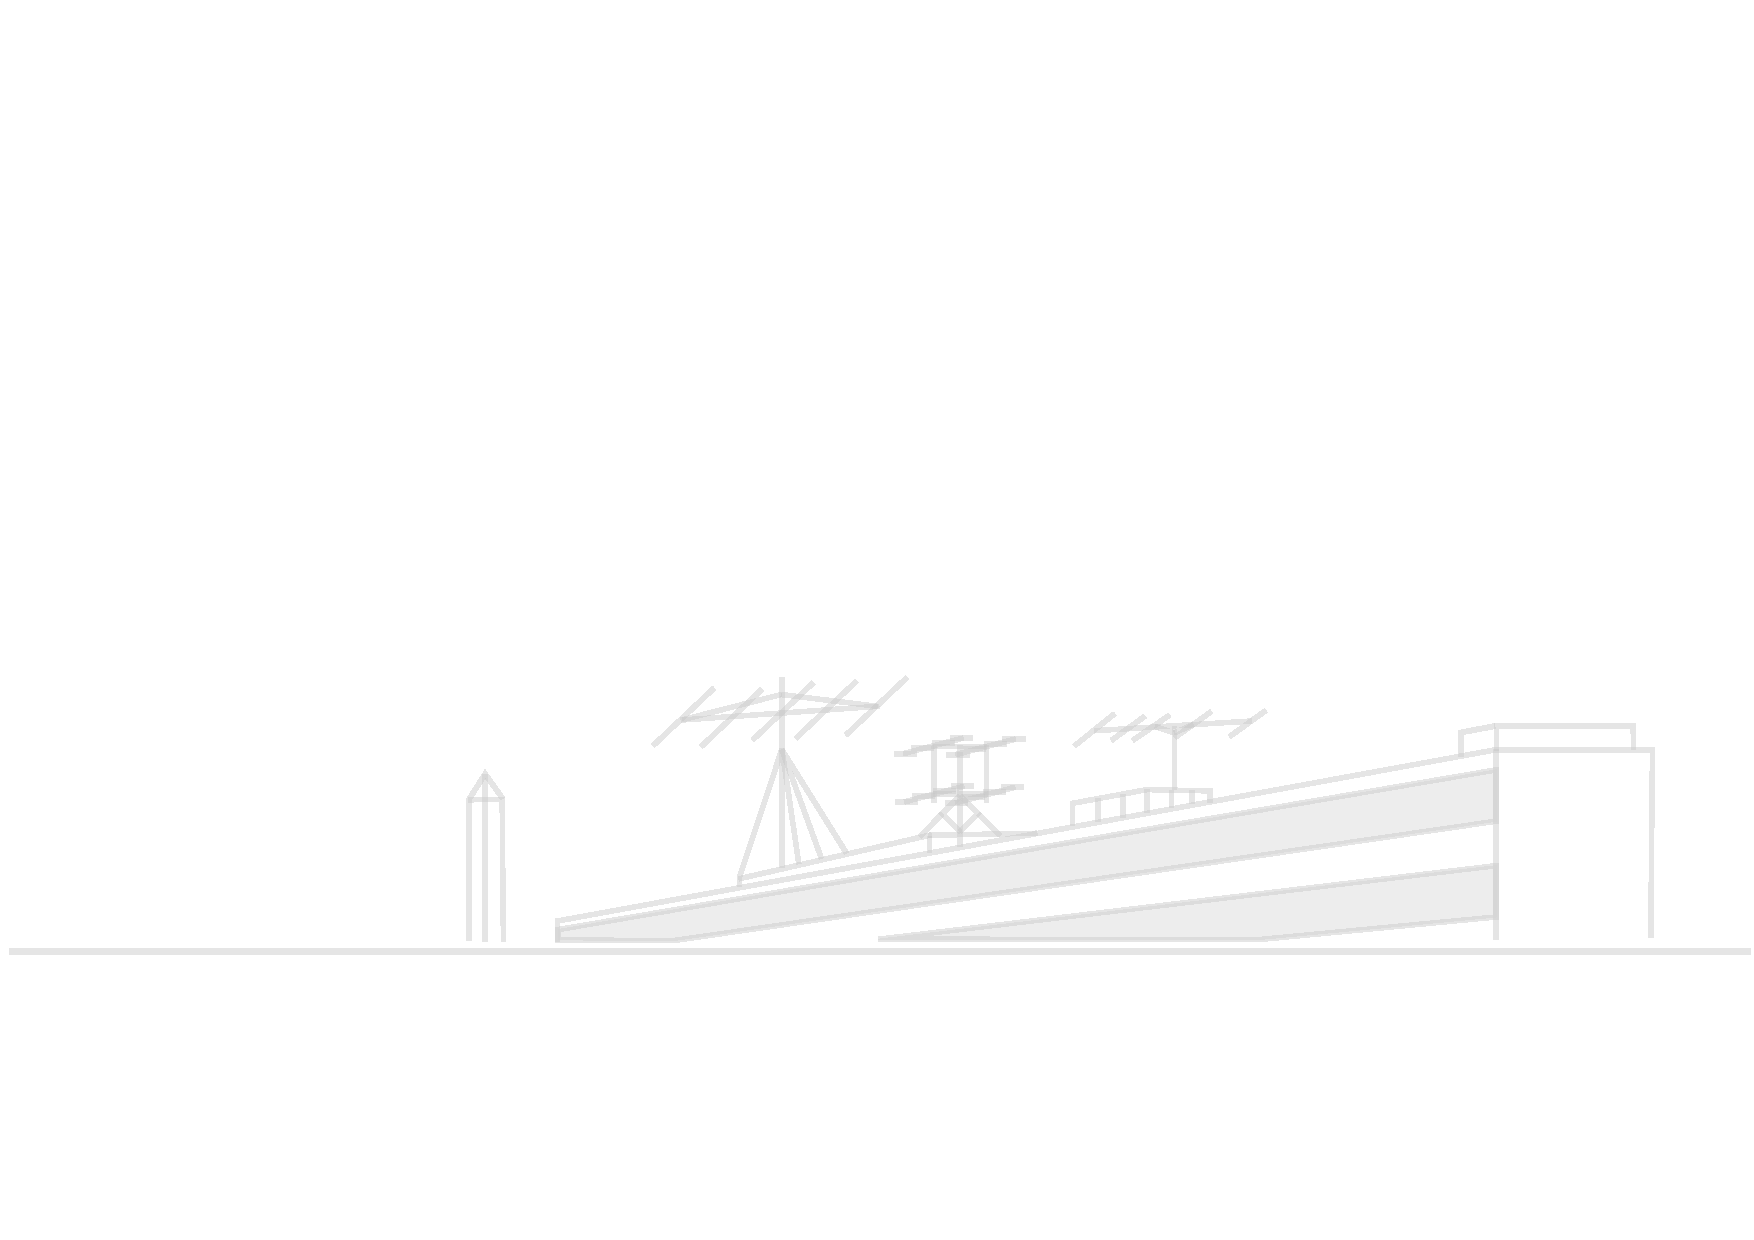
\includegraphics[width=17.8cm]{texdata/dk0tu_rooftop_background.pdf}
}

% Foliennummer einfügen
\setbeamertemplate{footline}[frame number]
%\setbeamertemplate{footline}{}

% Ändere das Zeichen vor jedem item
%\setbeamertemplate{itemize item}{\color{craneorange}$\blacktriangleright$}
%\setbeamertemplate{itemize subitem}{\color{craneorange}$\triangleright$}
%\setbeamertemplate{itemize subsubitem}{\color{craneorange}$\blacktriangleright$}

% Ändert die Blöcke 
\setbeamertemplate{blocks}[rounded][shadow=true]
% default | rounded [shadow=true|false]

%
% Eigene Kommandos
%

% Hack to get natbib and beamer working together. "The beamer user guide suggests
% that only the manual bibliography entry approach is supported"
% on some system it works out of the box, sometimes you need the hack :-(
% so check it --dl7bst
\ifdefined\newblock
    \relax
\else
    \newcommand{\newblock}{}
\fi

% \includedia command to generate png out of a dia file
% NEEDS installed dia and pdflatex option --shell-escape
\newcommand{\includedia}[1]{
    \immediate\write18{/usr/bin/dia #1.dia -e #1_diatmp.png -t png}
}

% RICHIG GROSSER FONT!
\newfont{\bigfont}{cmr10 at 144pt}
\newfont{\smallfont}{cmr10 at 8pt}

% Römische Ziffern
\makeatletter
\newcommand{\rmnum}[1]{\romannumeral #1}
\newcommand{\Rmnum}[1]{\expandafter\@slowromancap\romannumeral #1@}
\makeatother

% Schwarze Überschrift
%\setbeamercolor{frametitle}{fg=black}
%\setbeamercolor{title}{fg=black}

% Item- und Box-Farben
\definecolor{deepBlue}{HTML}{000066}
\setbeamercolor{itemize item}{fg=deepBlue}
\setbeamercolor{itemize subitem}{fg=deepBlue}
\setbeamercolor{description item}{fg=deepBlue}
\setbeamercolor{block title}{fg=deepBlue!100, bg=blue!15}
\setbeamercolor{block body}{fg=black, bg=blue!5}
\setbeamercolor{block title alerted}{fg=deepBlue, bg=red!75}
\setbeamercolor{block body alerted}{fg=black, bg=red!15}
\setbeamercolor*{block title example}{fg=blue!50, bg=blue!10}
\setbeamercolor*{block body example}{fg= blue, bg=blue!5}

%\setbeamercolor{section in head/foot}{parent=palette primary}
%\setbeamercolor{subsection in head/foot}{parent=palette secondary}
%\setbeamercolor{sidebar}{fg=darkblue,bg=yellow!90!orange}
%\setbeamercolor{title in sidebar}{fg=darkblue}
%\setbeamercolor{author in sidebar}{fg=darkblue}
%\setbeamercolor{section in sidebar}{fg=darkblue!10!black}
%\setbeamercolor{subsection in sidebar}{fg=darkblue!50!black}

% Titlepage Infos
\title{AFu-Kurs nach DJ4UF}
\author[DKØTU]{DKØTU\\ \footnotesize{Amateurfunkgruppe der TU Berlin}}
\institute[DKØTU]{\url{http://www.dk0tu.de} }

% PDF-Eigenschaften
\subject{DK0TU-Amateurfunkkurs nach DJ4UF}
\keywords{Amateurfunk Kurs HAM Radio Course CC-BY-NC-SA OpenSource TU Berlin DK0TU}

\subtitle{Technik Klasse A 10: \\
          HF-Leitungen \& Kabel \\[2em]}
\date{Stand 03.06.2016}
 \begin{document}

\begin{frame}
    \titlepage
    \vfill
    \begin{center}
        \ccbyncsaeu\\
        {\tiny This work is licensed under the \em{Creative Commons Attribution-NonCommercial-ShareAlike 3.0 License}.}\\[0.5ex]
         \tiny Amateurfunkgruppe der Technische Universität Berlin (AfuTUB), DKØTU
         %\includegraphics[scale=0.5]{img/DK0TU_Logo.pdf}
    \end{center}
\end{frame}


%fixme Referenzen/Fußnoten-Systematik vereinheitlichen

\section*{HF-Leitung}
\begin{frame}
  \frametitle{Hochfrequenzleitungen}
  \begin{center}
    %\begin{minipage}{0.4\textwidth}
    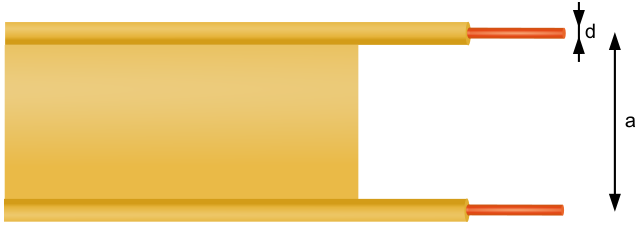
\includegraphics[width=\textwidth,height=.35\textheight,keepaspectratio]{a10/parallel.png}\\
    {\tiny Abb.1: Paralleldrahtleitung \cite{wp}}
    %\end{minipage}\\
    \\
    %\begin{minipage}{0.4\textwidth}
    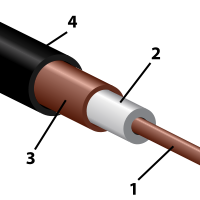
\includegraphics[width=\textwidth,height=.35\textheight,keepaspectratio]{a10/coax.png}\\
    {\tiny Abb.2: Koaxialkabel \cite{wm}}
    %\end{minipage}
  \end{center}
\end{frame}

\begin{frame}
  \frametitle{Hochfrequenzleitungen}
  \begin{center}
    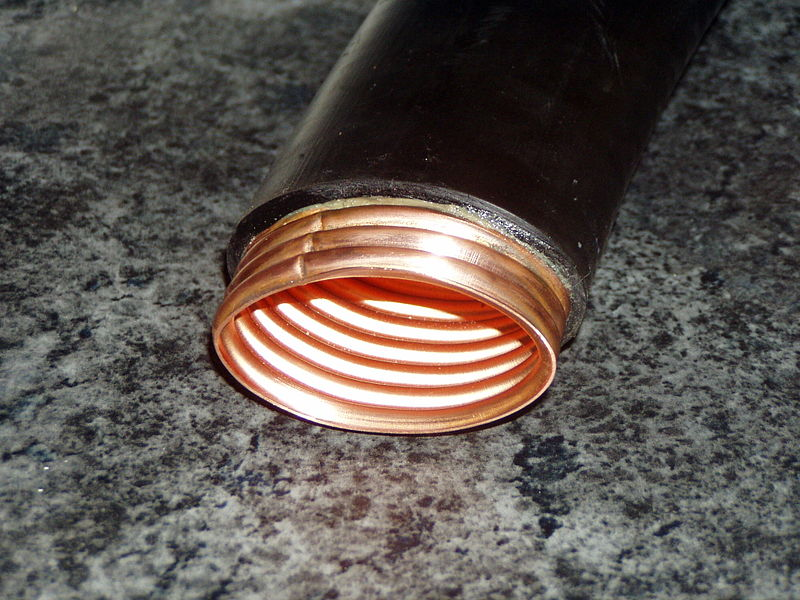
\includegraphics[width=\textwidth,height=.8\textheight,keepaspectratio]{a10/hohl.jpg}\\
    {\tiny Abb.3: Hohlleiter \cite{wp}}
    %\end{minipage}
  \end{center}
\end{frame}

\section*{Wellen"-widerstand}
\begin{frame}
  \frametitle{Wellenwiderstand}
  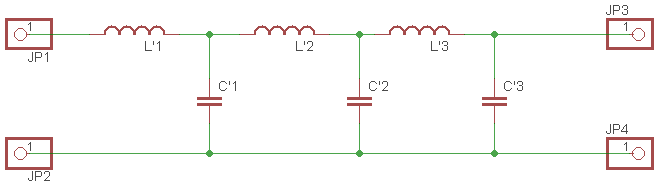
\includegraphics[width=\textwidth,height=.35\textheight,keepaspectratio]{a10/wellenesb.png}\\
  {\tiny Abb.4: ESB}
  \vspace{2em}\\
  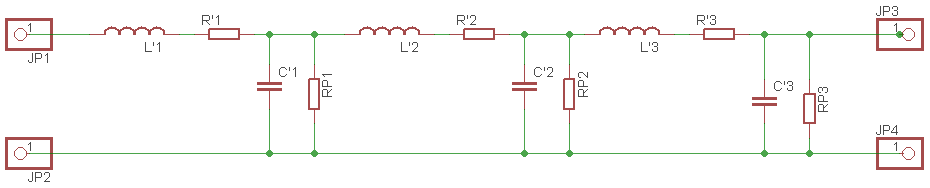
\includegraphics[width=\textwidth,height=.35\textheight,keepaspectratio]{a10/wellenesbex.png}\\
  {\tiny Abb.5: Genaues Ersatzschaltbild eines Koxialkabels}
\end{frame}

\begin{frame}
  \frametitle{Wellenwiderstand}
  \begin{itemize}
      \begin{block}{Wellenwiderstand}
        $Z_W = \sqrt{\cfrac{L'}{C'}}$
      \end{block}
    \item Paralleldrahtleitungen: $Z_W = 150 \Omega \text{ bis } 600 \Omega$
    \item Koaxialleitungen: $Z_W = 50 \Omega \text{ bis } 95 \Omega$
    \item Der Wellenwiderstand entspricht dem Abschlusswiderstand einer Leitung, bei dem keine stehenden Wellen auftreten.
  \end{itemize}
\end{frame}

\section*{Verkürzungs"-faktor}
\begin{frame}
  \frametitle{Verkürzungsfaktor}
  \begin{itemize}
    \item das Dielektrikum verlangsamt die Ausbreitungsgeschwindigkeit im Kabel: \\
          $v = \cfrac{1}{\sqrt{L' C'}}$
    \item durch geringere Ausbreitungsgeschwindigkeit verkürzt sich die
          Wellenlänge auf der Leitung: \\ $k = \cfrac{v}{c}$
  \end{itemize}
\end{frame}

\begin{frame}
  \frametitle{Typische Verkürzungsfaktoren}
  \begin{center}
    \begin{tabular}{l|l}
      \textbf{Kabeltyp} & \textbf{Verkürzungsfaktor} \\ \hline
      Koaxialkabel, normal & $k = 0,66$ \\
      Koaxialkabel mit Luftisolation & $k = 0,85$ \\
      offene $600 \Omega$ Speiseleitung & $k = 0,98$ \\
      Flachleitung mit $300 \Omega$ & $k = 0,82$ \\
    \end{tabular}
  \end{center}
\end{frame}

\section*{Skin-Effekt (Wdh.)}
\begin{frame}
  \frametitle{Der Skin-Effekt (Wiederholung aus A02)}
  \begin{itemize}
    \item tritt bei höherfrequenter Wechselspannung auf
    \item verdrängt Elektronen aus dem Leitungsinneren an die Leiteroberfläche \\
          $\rightarrow$ Widerstand im Leiter steigt
  \end{itemize}
\end{frame}

\begin{frame}
  \frametitle{Ursachen des Skin-Effektes}
  \begin{center}
    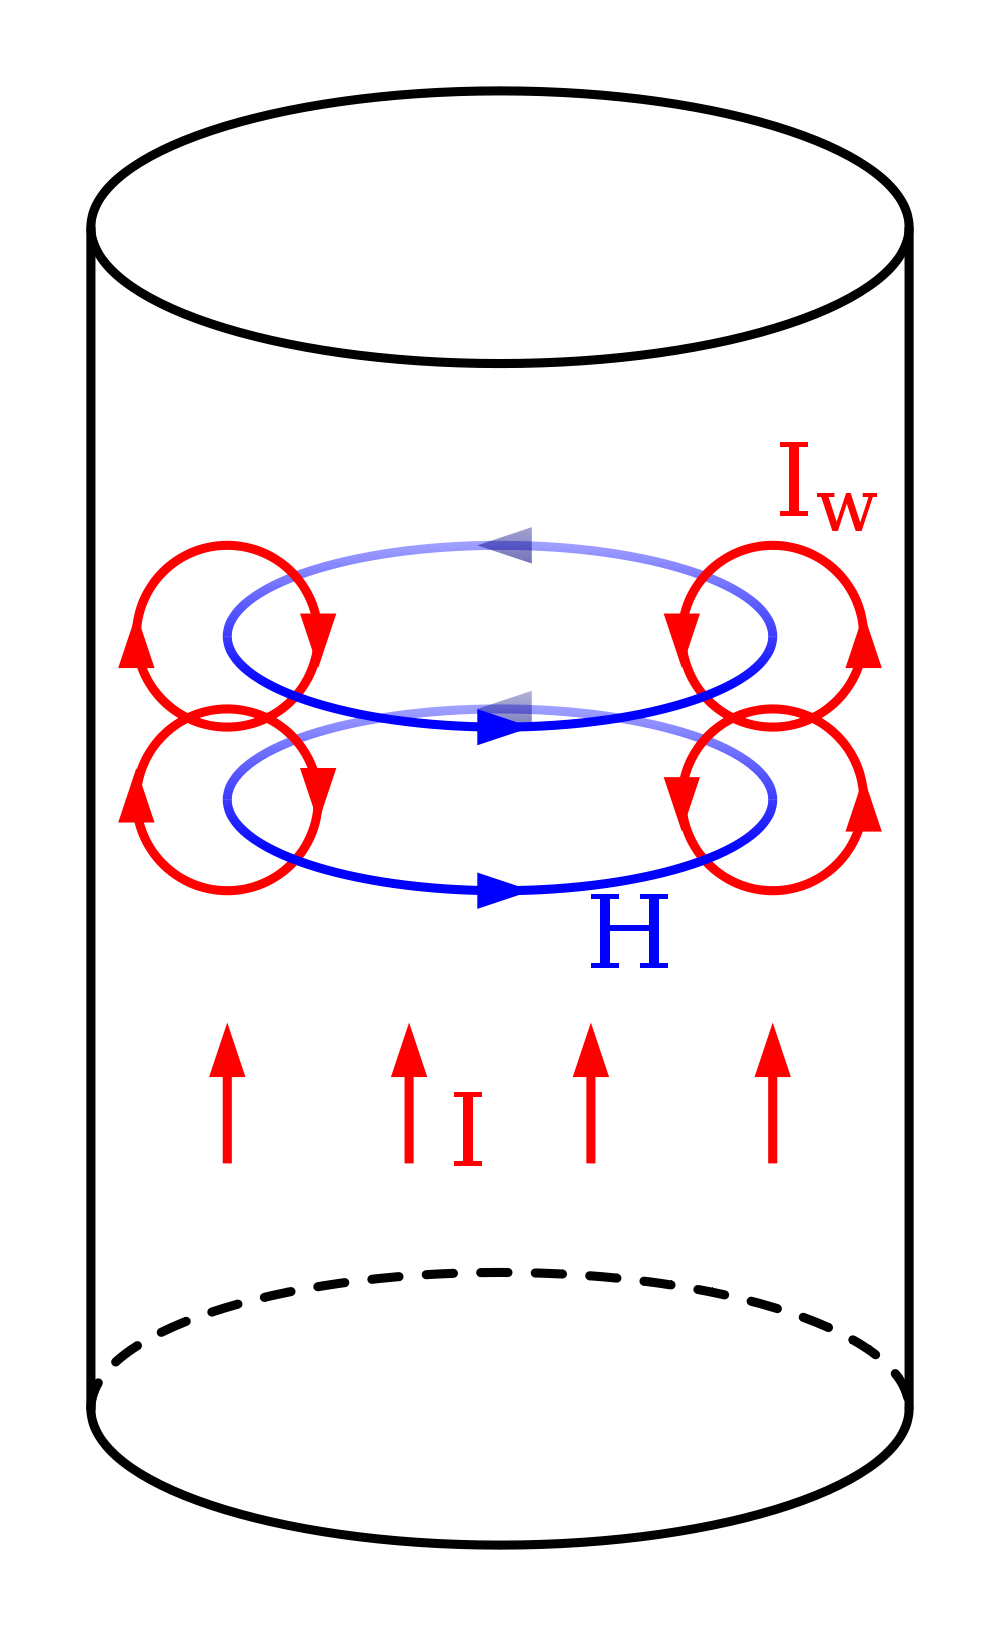
\includegraphics[width=.4\textwidth,height=.35\textheight,keepaspectratio]{a02/Skineffect.png}\\
    {\tiny Abb.5: Überlagerung von Wechsel- und Wirbelströmen \cite{wp}}
    \begin{itemize}
      \item Ursache des Skin-Effektes ist das magnetische Feld
      \item Es erzeugt Wirbelströme im Innern des Leiters
      \item Diese sind dem Erzeugerstrom entgegengerichtet
      \item Das wechselnde Magnetfeld erzeugt im Leiter eine höhere Gegenspannung als am Rand
    \end{itemize}
  \end{center}
\end{frame}

\begin{frame}
  \frametitle{Folgen \& Gegenmaßnahmen}
  \textbf{Folgen:}
  \begin{itemize}
    \item Der Leiterquerschnitt sinkt
    \item Die Impedanz steigt
  \end{itemize}
  \textbf{Gegenmaßnahmen}
  \begin{itemize}
    \item Verwendung von Hohlleitern
    \item Mehrere voneinander isolierte Drähte nutzen
    \item Oberfläche versilbern
  \end{itemize}
\end{frame}

\begin{frame}
  \begin{tabular}{l||p{.8\textwidth}}\hline
    \textbf{TC314} & \textbf{Welche Folgen hat der Skin-Effekt?}\\ \hline\hline
    A & Der Skin-Effekt ist für den mit der Frequenz ansteigenden induktiven Widerstand verantwortlich.\\ \hline
    B & Der Strom fließt bei hohen Frequenzen nur noch in der Oberfläche des Leiters. Mit sinkendem stromdurchflossenen Querschnitt steigt daher der induktive Widerstand des Leiters.\\ \hline
    C & Der Strom fließt bei hohen Frequenzen nur noch in der Oberfläche des  Leiters. Mit sinkendem stromdurchflossenen Querschnitt vergrößert sich daher der kapazitive Widerstand des Leiters.\\ \hline
    D \only<2>\checkmark & Der Strom fließt bei hohen Frequenzen nur noch in der Oberfläche des Leiters. Mit sinkendem stromdurchflossenen Querschnitt steigt daher der effektive Widerstand des Leiters.\\ \hline
  \end{tabular}
\end{frame}

\section*{D\"ampfung}
\begin{frame}
  \frametitle{Die Dämpfung}
  \begin{itemize}
    \item	Gibt den Leistungsverlust über das Kabel an
    \item	Hängt vom Verlustwiderstand und dem Dielektrikum ab
    \item	Wird meist in dB pro $100m$ angegeben
      \begin{Large}
      \item	$n = \sqrt{\cfrac{f_{hoch}}{f_{niedrig}}}$
      \end{Large}
  \end{itemize}
\end{frame}

\begin{frame}
    \frametitle{Kabeldämpfung Beispiel 1}
    
    \begin{exampleblock}{RG 213/U hat bei $100MHz$ eine Dämpfung von $6,7dB$.
                         Wie groß ist die Dämpfung bei $145MHz$?}
        \only<1>{Hinweis: $n = \sqrt{\cfrac{f_{hoch}}{f_{niedrig}}}$
                 \vspace{2em}}
        \only<2>{$n = \sqrt{\cfrac{f_2}{f_1}} = \sqrt{\cfrac{145}{100}} = \sqrt{1,45} = 1,2$ \\[1em]
                 Bei $145MHz$ ist die Dämpfung also: $1,2 \cdot 6,7dB = 8dB$
        }
    \end{exampleblock}

\end{frame}

\begin{frame}
  \frametitle{Kabeldämpfung Beispiel 2}

  % FIXME Musterloesungen mit rein!
  \begin{exampleblock}{Löse mit Hilfe des Dämpfungsdiagramms aus der Formelsammlung:}
    \begin{minipage}{0.3\textwidth}
      \begin{itemize}
        \item \textbf{RG58}\\
        \item 15 m\\
        \item 28 MHz
      \end{itemize}
    \end{minipage}
    \begin{minipage}{0.3\textwidth}
      \begin{itemize}
        \item \textbf{Aircell7}\\
        \item 15 m\\
        \item 28 MHz
      \end{itemize}
    \end{minipage}
    \begin{minipage}{0.3\textwidth}
      \begin{itemize}
        \item \textbf{RG174}\\
        \item 15 m\\
        \item 28 MHz
      \end{itemize}
    \end{minipage}
  \end{exampleblock}
\end{frame}

\section*{Steh"-wellen"-verh\"altnis (Wdh.)}
\begin{frame}
  \frametitle{Stehwellenverh\"altnis (Wiederholung)}
  \begin{itemize}
    \item ist ein Maß für die Anpassung
      \begin{Large}
        $SWR = s = \cfrac{U_{max}}{U_{min}}$
      \end{Large}
    \item	hängt vom Verhältnis Abschlusswiderstand $R_a$ zu Wellenwiderstand $Z_W$ ab \\
      \vspace{2mm}
      \begin{Large}
      $SWR = s = \cfrac{U_{max}}{U_{min}} = \frac{Z}{R_a} \text{ für } R_a \geq Z$
        \vspace{2mm}
      $SWR = s = \cfrac{U_{max}}{U_{min}} = \frac{R_a}{Z} \text{ für } Z \geq R_a$
      \end{Large}
      \vspace{2mm}
    \item ist das Verhältnis von vorlaufender zu zurücklaufender Welle
    \item \url{http://commons.wikimedia.org/wiki/File:Stehwelle_(Animation).gif}
  \end{itemize}
\end{frame}

\section*{Lecherleitung}
\begin{frame}
  \frametitle{Lecherleitung}
  \begin{center}
    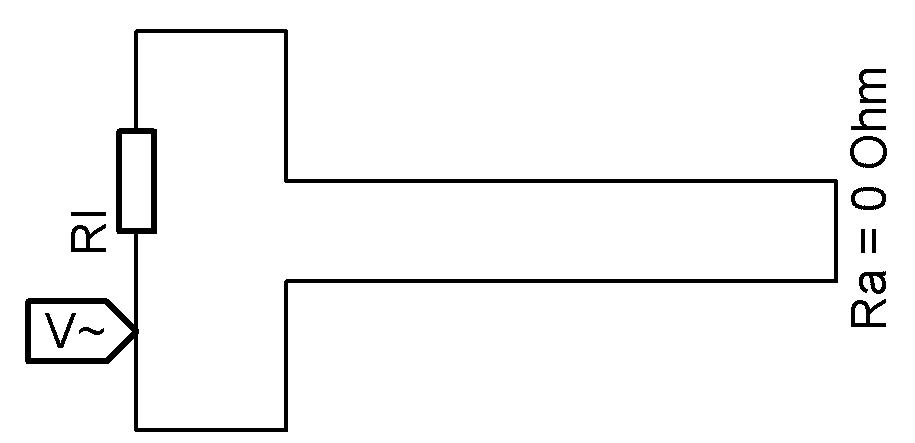
\includegraphics[width=\textwidth,height=.3\textheight,keepaspectratio]{a10/Lecherkreis.png}\\
    {\tiny Abb.6: Lecherkreis}
  \end{center}
  \begin{itemize}
    \item Ist ein Sonderfall einer Transformationsleitung mit einem Abschlusswiderstand von $0 \Omega$ oder $\infty \Omega$
    \item Gibt man HF-Signal auf Doppelleitung, mit $R_a = 0 \Omega$ wird die gesamte Energie reflektiert
    \item Dadurch entstehen Auslöschungen und Anhebungen
    \item Wellenwiderstand kehrt sich alle $\lambda /4$ um
    \item Lässt man das Leitungsende offen, kehren sich alle Verhältnisse um
    \item Dieser Effekt tritt auch bei einer $\lambda /2$ Leitung auf
  \end{itemize}
\end{frame}

\begin{frame}
    \frametitle{Lecherleitung}

    Zusammenfassung:
    
    \begin{itemize}
        \item	$\lambda /4$ Leitung kehrt Impedanzverhältnisse um (niederohmig $\leftrightarrow$ hochohmig), wirkt wie Schwingkreis
        \item	$\lambda /2$ Leitung transformiert 1:1, wirkt auch wie ein Schwingkreis
    \end{itemize}

\end{frame}

\begin{frame}
  \begin{tabular}{l||p{.8\textwidth}}\hline
    \textbf{TH325} & \textbf{Eine Lecherleitung besteht aus zwei parallelen Leitern. Wovon ist ihre Resonanzfrequenz wesentlich abhängig? Sie ist abhängig}\\ \hline\hline
    A & vom verwendeten Abschlusswiderstand. \\ \hline
    B \only<2>\checkmark & von der Leitungslänge \\ \hline
    C & vom Wellenwiderstand der beiden parallelen Leiter. \\ \hline
    D & vom Leerlauf-Kurzschlussverhalten. \\ \hline
  \end{tabular}
\end{frame}

\begin{frame}
  \begin{tabular}{l||p{.8\textwidth}}\hline
    \textbf{TH326} & 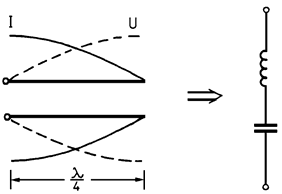
\includegraphics[width=\textwidth,height=.3\textheight,keepaspectratio]{a10/th326.png}\\
    & \textbf{Was zeigt diese Darstellung?}\\ \hline\hline
    A & Sie zeigt die Strom- und Spannungsverteilung an einer Antennenspeiseleitung. Die Antenne arbeitet als Serienresonanzkreis. \\ \hline
    B & Sie zeigt die Strom- und Spannungsverteilung an den Radialen einer Groundplane. Die Antenne arbeitet mit Verlängerungsspule zur Resonanzanpassung.\\ \hline
    C & Sie zeigt die Strom- und Spannungsverteilung an einer Antenne. Die Antenne arbeitet als Groundplane mit Verkürzungskondensator. \\ \hline
    D \only<2>\checkmark & Sie zeigt die Strom- und Spannungsverteilung an einer offenen $\lambda/4$-Lecherleitung. Sie wirkt als Reihenschwingkreis. \\ \hline
  \end{tabular}
\end{frame}

\section*{Trans"-formations"-leitungen}
\begin{frame}
  \frametitle{Transformationsleitungen}
  \begin{itemize}
    \item dienen der Anpassung von Antenne zum Sender, dazu \dots
    \begin{itemize}
        \item Anpassung des Sender-Widerstandes an die HF-Leitung
        \item Anpassung der Antennenimpedanz an das Kabel
    \end{itemize}
    \item $R_i = Z_w = Z_{Antenne}$
  \end{itemize}
\end{frame}

\begin{frame}
  \frametitle{Prinzip der Transformationsleitung}
  \begin{center}
    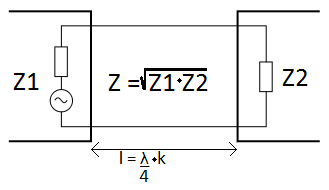
\includegraphics[width=\textwidth,height=.35\textheight,keepaspectratio]{a10/Anpassung.png}\\
    {\tiny Abb.7: Anpassung \cite{wp}}
  \end{center}
  \begin{itemize}
    \item	Eine $\lambda /4$-Leitung kann Widerstände tranformieren
    \item	Aber nur in einer begrenzten Bandbreite
    \item	Leitung wirkt als Transformator
    \item	Eine solche Leitung bestimmter Länge auch als abgestimmte Speiseleitung bezeichnet
    \item	Leitungen die mit ihrem Wellenwiderstand abgeschlossen werden, um Stehwellen zu vermeiden, nennt man unabgestimmte Speiseleitung
  \end{itemize}
\end{frame}

\begin{frame}

    Will man zwei Impedanzen $Z_E$ \& $Z_A$ mit einem Viertelwellentransformator
    anpassen, so muss die Transformationsleitung folgende Werte besitzen:

  \begin{itemize}
    \item	Wellenwiderstand:\\
      \vspace{2mm}
      \begin{Large}
        $Z = \sqrt{Z_E \cdot Z_A}$
      \end{Large}
      \vspace{2mm}
    \item	Länge: \\
      \vspace{2mm}
      \begin{Large}
        $\ell = (2n - 1) \cdot \frac{\lambda}{4} \cdot k$
      \end{Large}
      \vspace{3mm}
    \item	Bei Koaxialkabeln sieht das Ganze wie folgt aus:
      \vspace{3mm}
      \begin{align*}
         Z &= \frac{60 \Omega}{\sqrt{\varepsilon_r}} \cdot ln(\frac{D}{d}) \\
           &= \frac{138 \Omega}{\sqrt{\varepsilon_r}} \cdot lg(\frac{D}{d})
      \end{align*}
  \end{itemize}
\end{frame}

\section*{Symmetrierung}
\begin{frame}
  \frametitle{Symmetrierung}
  \begin{minipage}{0.3\textwidth}
    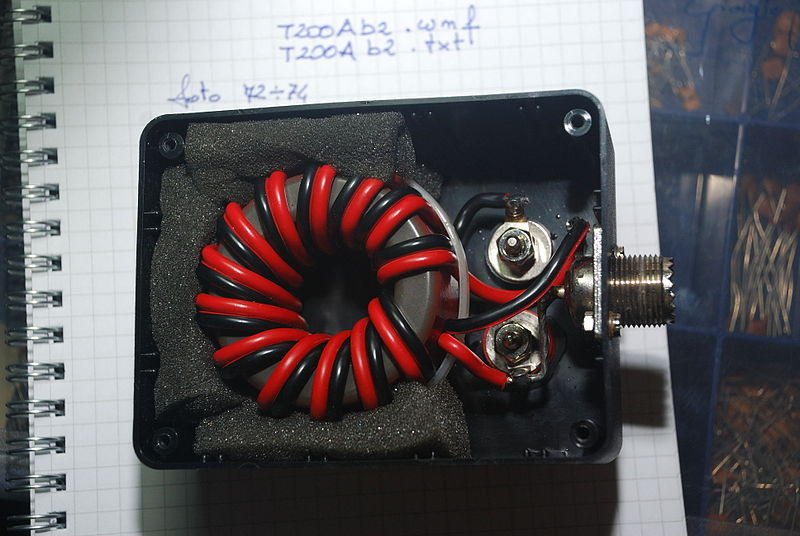
\includegraphics[width=\textwidth,height=.8\textheight,keepaspectratio]{a10/balun.jpg}\\
    {\tiny Abb.8: Balun \cite{wp}}
  \end{minipage}
  \hspace{2mm}
  \begin{minipage}{0.5\textwidth}
    \begin{itemize}
      \item Wird bei Verbindungen zwischen symmetrischen und unsymmetrischen Punkten verwendet
      \item Koaxialkabel ist unsymmetrisch
      \item Paralleldraht ist symmetrisch
      \item Alle Dipole sind symmetrisch
      \item Alle Antennen, die gegen Erde erregt werden sind unsymmetrisch
      \item	Ohne Symmetrierung entstehen Mantelwellen
    \end{itemize}
  \end{minipage}
\end{frame}

\begin{frame}
  \frametitle{Balun}
  \begin{center}
    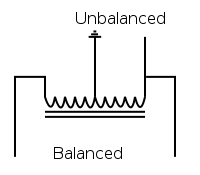
\includegraphics[height=.6\textheight,width=\textwidth,keepaspectratio]{a10/balun.png}\\
    {\tiny Abb.9: Spartrafo als Balun \cite{wm}}
  \end{center}
  \begin{itemize}
    \item	Balun kann symmetrieren und gleichzeitig die Impedanz anpassen
    \item	Wird der Eingang an halber Windungszahl des Ausganges angeschlossen, erhält man einen 1:4 Übertrager
  \end{itemize}
\end{frame}

\begin{frame}
  \frametitle{Die $\lambda /2$-Umwegleitung}
  \begin{minipage}{0.3\textwidth}
    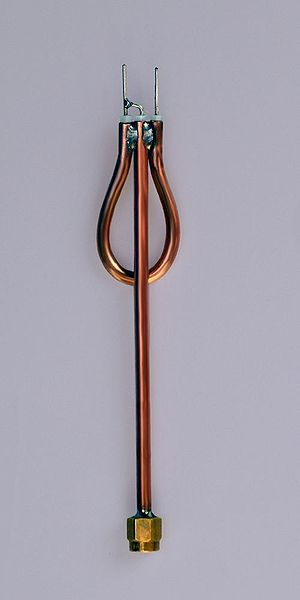
\includegraphics[height=.8\textheight,width=\textwidth,keepaspectratio]{a10/Umwegleitung.jpg}\\
    {\tiny Abb.10: $\lambda /2$-Umwegleitung \cite{wp}}
  \end{minipage}
  \hspace{2mm}
  \begin{minipage}{0.5\textwidth}
    \begin{itemize}
      \item An der Einspeisestelle teilt sich der Strom je zur Hälfte auf
      \item Eine Hälfte geht direkt zum Strom, die andere in die Umwegleitung
      \item Nach dem ohmschen Gesetz verdoppelt sich dadurch der Widerstand
      \item Bei $50 \Omega$ ergeben sich also $100 \Omega$
      \item Die Umwegleitung stellt den Widerstand auf der anderen Seite nochmal mit $100 \Omega$ zur Verfügung
      \item Somit ergeben sich insgesamt $200 \Omega$ Impedanz an der Antenne
    \end{itemize}
  \end{minipage}
\end{frame}

\section*{Topfkreis}
\begin{frame}
  \frametitle{Der Topfkreis}
  \begin{columns}
    \column[c]{.3\textwidth}
    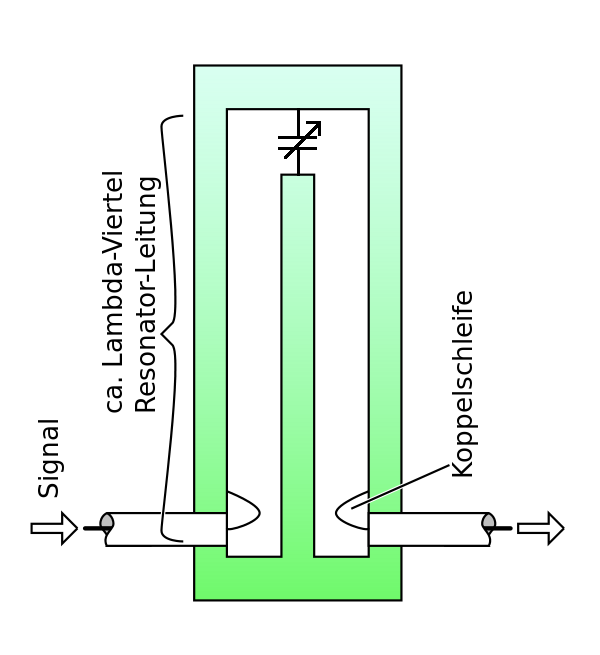
\includegraphics[width=\textwidth,height=.4\textheight,keepaspectratio]{a10/Topfkreis.png}\\
    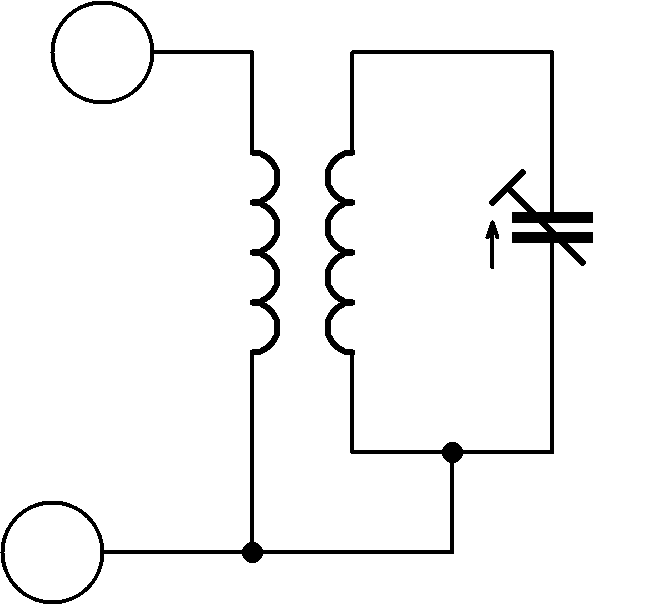
\includegraphics[width=\textwidth,height=.4\textheight,keepaspectratio]{a10/Topfkreis-ESB.png}\\
    {\tiny Abb.11: Topfkreis und ESB}
    \column{.65\textwidth}
    \begin{itemize}
      \item Im UHF-Bereich werden auch Aluminium- oder versilberte Messingbecher als Leiter genutzt
      \item Sie besitzen einen Mittelleiter, wodurch sie wie eine Koaxleitung wirken
      \item Sie lassen sich wie auch die Lecherleitung durch einen Kurzschlussschieber abstimmen
      \item Dieser Schwingkreis ist vollkommen abgestimmt und von außen nicht beeinflussbar
      \item Versilbert man die Innenflächen, lassen sich die Verlust minimieren
      \item Dadurch werden auch die elektrischen Eigenschaften für hohe Frequenzen verbessert
    \end{itemize}
  \end{columns}
\end{frame}

\begin{frame}
  \begin{exampleblock}{Hausaufgabe}
    Kapitel 1.8.3 Übertragungsleitungen mit Fragen TH301--TH331.\\
    Kapitel 1.8.4 Anpassung, Transformation und Symmetrierung mit Fragen TH401--TH423.\\
  \end{exampleblock}
\end{frame}

\renewcommand{\refname}{Referenzen}

\hypertarget{refs}{}
\textcolor{white}{} \\ %\vspace{} geht nicht
\Large Referenzen/Links
\footnotesize

\begin{thebibliography}{}
  \bibitem{wp}    Wikipedia - Die freie Enzyklopädie:
    \url{http://de.wikipedia.org/wiki/Datei:Twin-lead_cable_dimension.svg}
    \url{http://de.wikipedia.org/wiki/Datei:Elli_holl.jpg}
    \url{http://de.wikipedia.org/wiki/Datei:EingangswiderstandAusgangswiderstandA.svg}
    \url{http://de.wikipedia.org/wiki/Datei:Topfkreis_filter.svg}
    \url{http://de.wikipedia.org/wiki/Datei:EingangswiderstandAusgangswiderstandA.svg}
    \url{http://de.wikipedia.org/wiki/Datei:T200A2.jpg}
    \url{http://de.wikipedia.org/wiki/Datei:Balun(semirigid).jpg}
  \bibitem{darc}  DARC Online-Lehrgang Lektion A08:
    \url{http://www.darc.de/referate/ajw/ausbildung/darc-online-lehrgang/technik-klasse-a/technik-a10/}
  \bibitem{wm} 	Wikimedia:
    \url{http://commons.wikimedia.org/wiki/File:Coaxial_cable_cutaway_new.svg}
    \url{http://commons.wikimedia.org/wiki/File:Cdbalun2.svg}
  \bibitem{bna}   Fragenkatalog Bundesnetzagentur Technik Klasse A:
    \mbox{\url{https://www.bundesnetzagentur.de/SharedDocs/Downloads/DE/Sachgebiete/Telekommunikation/Unternehmen_Institutionen/Frequenzen/Amateurfunk/Fragenkatalog/TechnikFragenkatalogKlasseAf252rId9014pdf.pdf?__blob=publicationFile&v=3}}
\end{thebibliography}

% Hier könnte noch eine Kontaktfolie stehen

\end{document}

